\documentclass[tikz, border=3pt]{standalone}
\usepackage{tikz}
\usetikzlibrary{
    positioning, 
    arrows.meta, 
    decorations.pathreplacing, 
    calc
}

\begin{document}
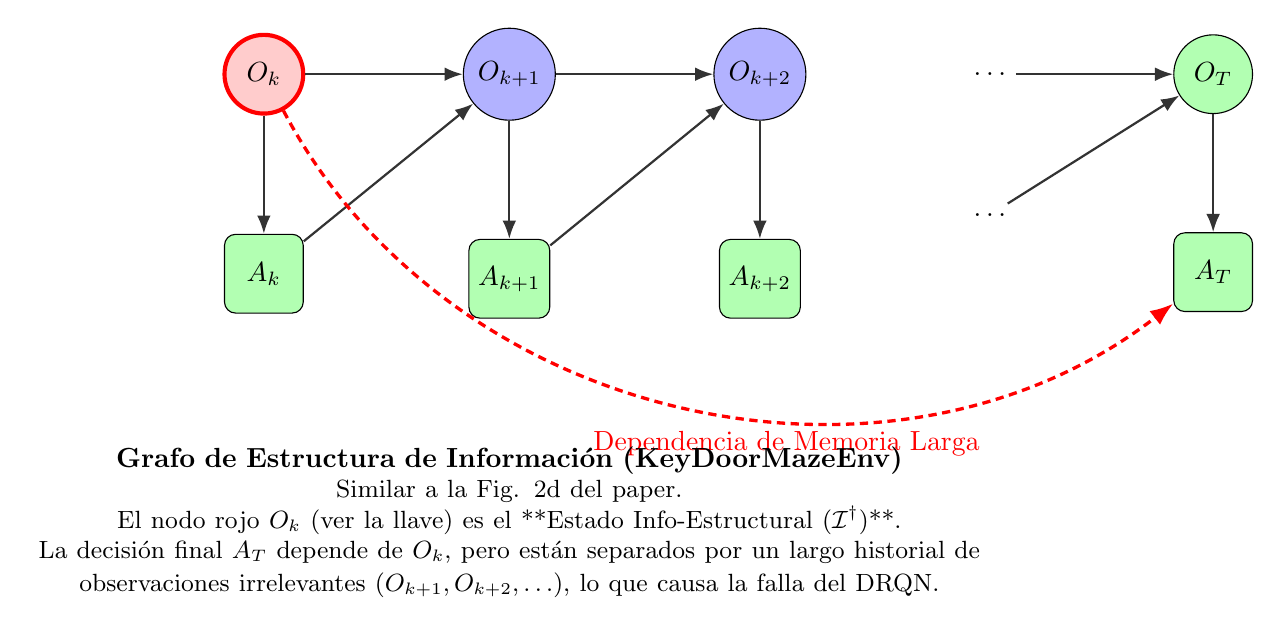
\begin{tikzpicture}[
    node distance=1.5cm and 2cm,
    % Estilos de Nodos (como en Página 7)
    past_obs/.style={circle, draw=black, fill=blue!30, minimum size=1cm},
    past_act/.style={rectangle, draw=black, fill=green!30, minimum size=1cm, rounded corners},
    future_obs/.style={circle, draw=black, fill=green!30, minimum size=1cm},
    future_act/.style={rectangle, draw=black, fill=green!30, minimum size=1cm, rounded corners},
    critical_node/.style={circle, draw=red, fill=red!20, minimum size=1cm, line width=1.5pt}, % El nodo rojo
    % Estilos de Flechas
    arrow/.style={-Latex, thick, draw=black!80},
    long_arrow/.style={-Latex, thick, draw=red, densely dashed, very thick} % La flecha de memoria
]
% --- PASADO (t=k, ves la llave) ---
\node[critical_node] (obs_k) {$O_k$};
\node[past_act] (act_k) [below=of obs_k] {$A_k$};
\draw[arrow] (obs_k) -- (act_k);

% --- PASADO (t=k+1, pasillo) ---
\node[past_obs] (obs_k1) [right=of obs_k, node distance=4cm] {$O_{k+1}$};
\node[past_act] (act_k1) [below=of obs_k1] {$A_{k+1}$};
\draw[arrow] (obs_k1) -- (act_k1);
\draw[arrow] (act_k) -- (obs_k1);
\draw[arrow] (obs_k) -- (obs_k1);

% --- PASADO (t=k+2, pasillo) ---
\node[past_obs] (obs_k2) [right=of obs_k1, node distance=4cm] {$O_{k+2}$};
\node[past_act] (act_k2) [below=of obs_k2] {$A_{k+2}$};
\draw[arrow] (obs_k2) -- (act_k2);
\draw[arrow] (act_k1) -- (obs_k2);
\draw[arrow] (obs_k1) -- (obs_k2);

% --- PUNTOS SUSPENSIVOS (...) ---
\node (dots) [right=of obs_k2, node distance=3cm] {$\dots$};
\node (dots_a) [below=of dots] {$\dots$};

% --- PRESENTE (t=T, en la puerta) ---
\node[future_obs] (obs_T) [right=of dots, node distance=3cm] {$O_T$};
\node[future_act] (act_T) [below=of obs_T] {$A_T$};
\draw[arrow] (obs_T) -- (act_T);
\draw[arrow] (dots) -- (obs_T);
\draw[arrow] (dots_a) -- (obs_T);

% --- LA FLECHA CRÍTICA DE MEMORIA (La d-separación) ---
% La acción A_T depende de la observación actual O_T,
% pero también de la observación lejana O_k (la llave).
% Esta es la dependencia que el LSTM "olvida".
\draw[long_arrow] (obs_k) to [bend right=50] node[pos=0.6, below, text=red] {Dependencia de Memoria Larga} (act_T);


% --- Leyenda ---
\node [text=black, text width=12cm, align=center,
       below=of act_k1, node distance=3.5cm] 
    {
    \textbf{Grafo de Estructura de Información (KeyDoorMazeEnv)} \par
    \small
    Similar a la Fig. 2d del paper. \par
    El nodo rojo $O_k$ (ver la llave) es el **Estado Info-Estructural ($\mathcal{I}^\dagger$)**. \par
    La decisión final $A_T$ depende de $O_k$, pero están separados por un largo historial de \par
    observaciones irrelevantes ($O_{k+1}, O_{k+2}, \dots$), lo que causa la falla del DRQN.
    };

\end{tikzpicture}
\end{document}